\documentclass[tikz,border=12pt]{standalone}
\usepackage[T1]{fontenc}
\usepackage{tgheros}
\usepackage{sfmath}
\usepackage{amsmath,amssymb}
% % \usepackage{fontawesome5} (Removed for publication-grade academic typography) (Removed for publication-grade academic typography)
\usepackage{tikz}
\usetikzlibrary{arrows.meta,positioning,shapes.geometric,fit,backgrounds,calc}
\usepackage{xcolor}

\renewcommand{\familydefault}{\sfdefault}

% Canonical Semantic Palette
\definecolor{structuralnavy}{HTML}{1B2A4A}
\definecolor{measuredteal}{HTML}{168F84}
\definecolor{proposalamber}{HTML}{C98218}
\definecolor{consequencecoral}{HTML}{BD4F2F}
\definecolor{authorityviolet}{HTML}{6550A8}
\definecolor{neutralgray}{HTML}{687386}
\definecolor{navyfill}{HTML}{E8EDF6}
\definecolor{tealfill}{HTML}{E4F6F3}
\definecolor{amberfill}{HTML}{FFF3DC}
\definecolor{coralfill}{HTML}{FAE9E2}
\definecolor{grayfill}{HTML}{F4F6F7}
\definecolor{cardborder}{HTML}{CBD5E1}

\begin{document}
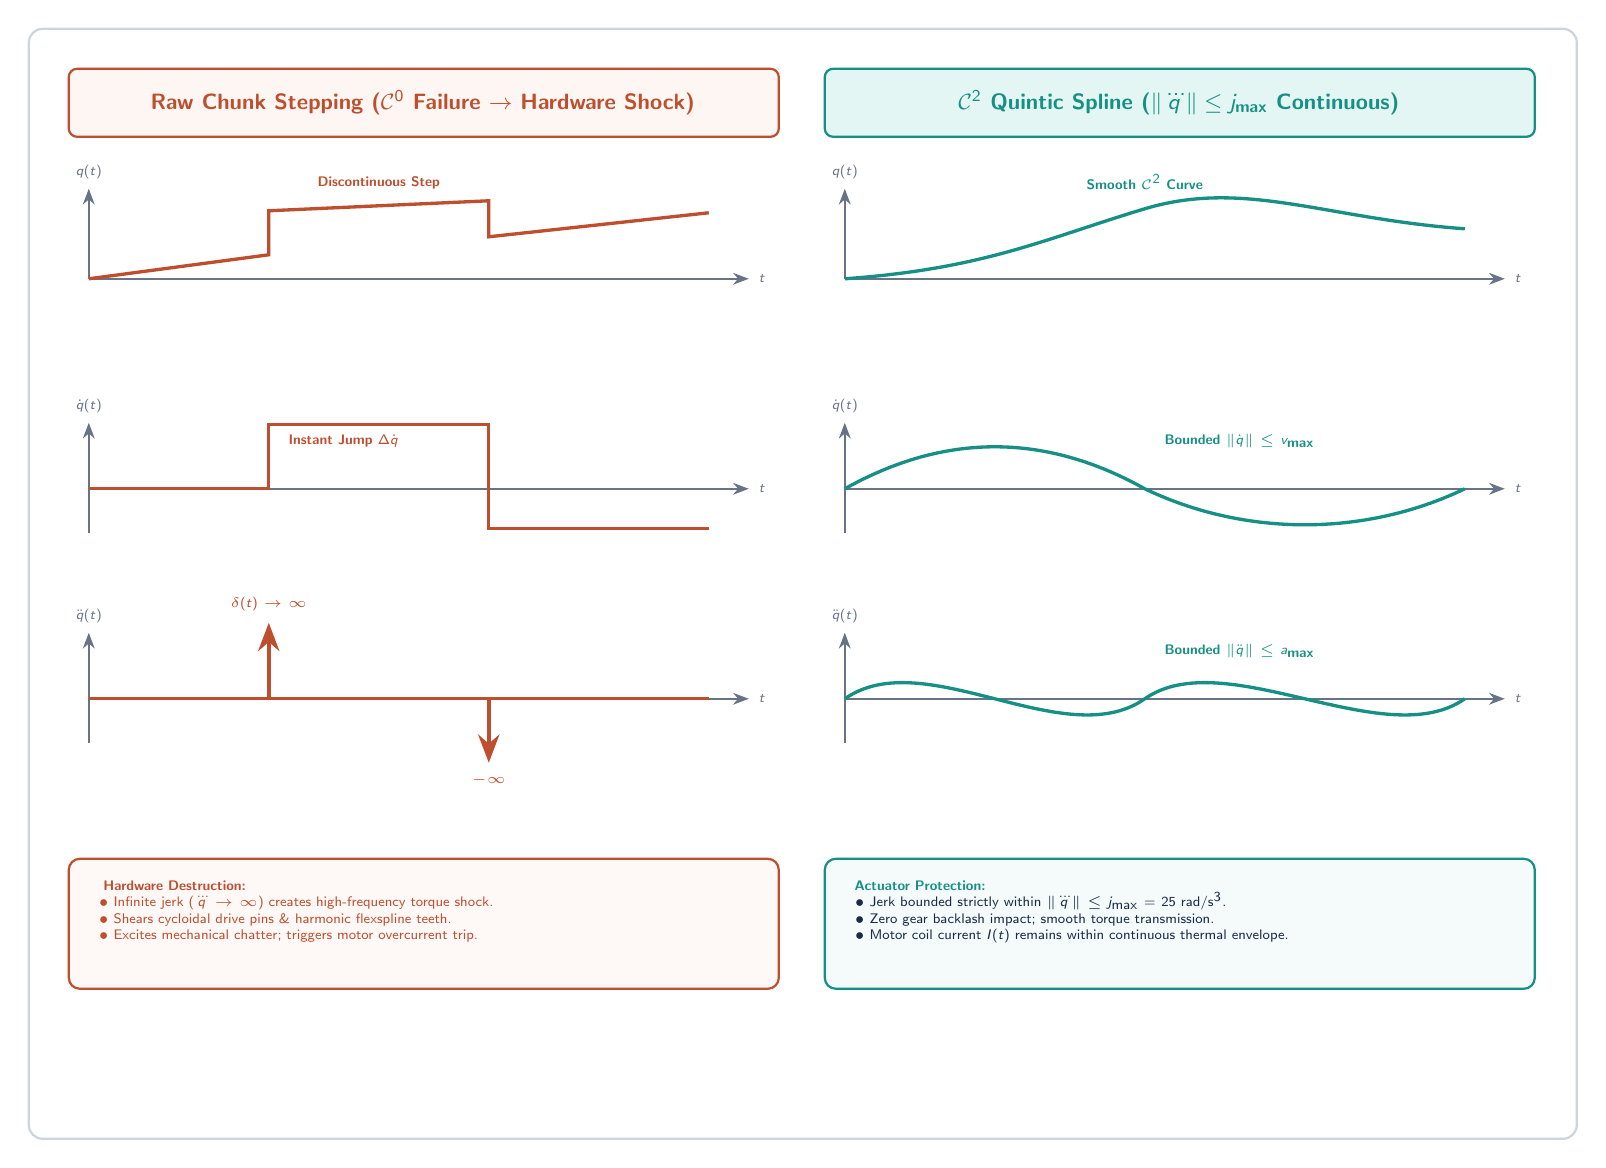
\begin{tikzpicture}[
  font=\sffamily,
  >=Stealth,
  card/.style={
    draw=cardborder,
    fill=white,
    rounded corners=5pt,
    line width=0.8pt,
    inner sep=8pt
  }
]

  % Main Container Card
  \coordinate (c_top) at (0, 0);
  \draw[draw=cardborder, fill=white, rounded corners=5pt, line width=0.8pt] 
    (c_top) rectangle ++(7.74in, -5.55in);

  % ----------------------------------------------------
  % COLUMN HEADERS
  % ----------------------------------------------------
  \coordinate (col_left) at ($(c_top) + (0.2in, -0.20in)$);
  \draw[draw=consequencecoral, fill=coralfill!40, rounded corners=3pt, line width=0.8pt]
    (col_left) rectangle ++(3.55in, -0.34in);
  \node[font=\footnotesize\bfseries, color=consequencecoral] at ($(col_left) + (1.77in, -0.17in)$) {
     Raw Chunk Stepping ($\mathcal{C}^0$ Failure $\to$ Hardware Shock)
  };

  \coordinate (col_right) at ($(c_top) + (3.98in, -0.20in)$);
  \draw[draw=measuredteal, fill=tealfill, rounded corners=3pt, line width=0.8pt]
    (col_right) rectangle ++(3.55in, -0.34in);
  \node[font=\footnotesize\bfseries, color=measuredteal] at ($(col_right) + (1.77in, -0.17in)$) {
     $\mathcal{C}^2$ Quintic Spline ($\|\dddot{q}\| \le j_{\text{max}}$ Continuous)
  };

  % ----------------------------------------------------
  % ROW 1: Position q(t)
  % ----------------------------------------------------
  \coordinate (r1_left) at ($(col_left) + (0.1in, -1.05in)$);
  \draw[->, line width=0.6pt, neutralgray] (r1_left) -- ++(3.3in, 0) node[right, font=\tiny] {$t$};
  \draw[->, line width=0.6pt, neutralgray] (r1_left) -- ++(0, 0.45in) node[above, font=\tiny] {$q(t)$};
  % Step / piecewise linear position
  \draw[line width=1.2pt, consequencecoral] 
    (r1_left) -- ++(0.9in, 0.12in) -- ++(0, 0.22in) -- ++(1.1in, 0.05in) -- ++(0, -0.18in) -- ++(1.1in, 0.12in);
  \node[anchor=south, font=\tiny\bfseries, color=consequencecoral] at ($(r1_left) + (1.45in, 0.40in)$) {Discontinuous Step};

  \coordinate (r1_right) at ($(col_right) + (0.1in, -1.05in)$);
  \draw[->, line width=0.6pt, neutralgray] (r1_right) -- ++(3.3in, 0) node[right, font=\tiny] {$t$};
  \draw[->, line width=0.6pt, neutralgray] (r1_right) -- ++(0, 0.45in) node[above, font=\tiny] {$q(t)$};
  % Smooth quintic curve
  \draw[line width=1.2pt, measuredteal] 
    (r1_right) .. controls ++(0.7in, 0.05in) and ++(-0.5in, -0.15in) .. 
    ($(r1_right) + (1.5in, 0.35in)$) .. controls ++(0.5in, 0.15in) and ++(-0.7in, 0.05in) .. 
    ($(r1_right) + (3.1in, 0.25in)$);
  \node[anchor=south, font=\tiny\bfseries, color=measuredteal] at ($(r1_right) + (1.5in, 0.40in)$) {Smooth $\mathcal{C}^2$ Curve};

  % ----------------------------------------------------
  % ROW 2: Velocity q_dot(t)
  % ----------------------------------------------------
  \coordinate (r2_left) at ($(r1_left) + (0, -1.05in)$);
  \draw[->, line width=0.6pt, neutralgray] (r2_left) -- ++(3.3in, 0) node[right, font=\tiny] {$t$};
  \draw[->, line width=0.6pt, neutralgray] ($(r2_left) + (0, -0.22in)$) -- ++(0, 0.55in) node[above, font=\tiny] {$\dot{q}(t)$};
  % Discontinuous velocity jumps
  \draw[line width=1.2pt, consequencecoral] 
    (r2_left) -- ++(0.9in, 0) -- ++(0, 0.32in) -- ++(1.1in, 0) -- ++(0, -0.52in) -- ++(1.1in, 0);
  \node[anchor=west, font=\tiny\bfseries, color=consequencecoral] at ($(r2_left) + (0.95in, 0.24in)$) {Instant Jump $\Delta \dot{q}$};

  \coordinate (r2_right) at ($(r1_right) + (0, -1.05in)$);
  \draw[->, line width=0.6pt, neutralgray] (r2_right) -- ++(3.3in, 0) node[right, font=\tiny] {$t$};
  \draw[->, line width=0.6pt, neutralgray] ($(r2_right) + (0, -0.22in)$) -- ++(0, 0.55in) node[above, font=\tiny] {$\dot{q}(t)$};
  % Smooth continuous velocity
  \draw[line width=1.2pt, measuredteal] 
    (r2_right) .. controls ++(0.5in, 0.28in) and ++(-0.5in, 0.28in) .. 
    ($(r2_right) + (1.5in, 0)$) .. controls ++(0.5in, -0.24in) and ++(-0.5in, -0.24in) .. 
    ($(r2_right) + (3.1in, 0)$);
  \node[anchor=west, font=\tiny\bfseries, color=measuredteal] at ($(r2_right) + (1.55in, 0.24in)$) {Bounded $\|\dot{q}\| \le v_{\text{max}}$};

  % ----------------------------------------------------
  % ROW 3: Acceleration q_ddot(t) & Jerk q_dddot(t)
  % ----------------------------------------------------
  \coordinate (r3_left) at ($(r2_left) + (0, -1.05in)$);
  \draw[->, line width=0.6pt, neutralgray] (r3_left) -- ++(3.3in, 0) node[right, font=\tiny] {$t$};
  \draw[->, line width=0.6pt, neutralgray] ($(r3_left) + (0, -0.22in)$) -- ++(0, 0.55in) node[above, font=\tiny] {$\ddot{q}(t)$};
  % Delta spikes for acceleration
  \draw[line width=1.2pt, consequencecoral] (r3_left) -- ++(0.9in, 0);
  \draw[->, line width=1.6pt, consequencecoral] ($(r3_left) + (0.9in, 0)$) -- ++(0, 0.38in) 
    node[above, font=\tiny\bfseries] {$\delta(t) \to \infty$};
  \draw[line width=1.2pt, consequencecoral] ($(r3_left) + (0.9in, 0)$) -- ++(1.1in, 0);
  \draw[->, line width=1.6pt, consequencecoral] ($(r3_left) + (2.0in, 0)$) -- ++(0, -0.32in) 
    node[below, font=\tiny\bfseries] {$-\infty$};
  \draw[line width=1.2pt, consequencecoral] ($(r3_left) + (2.0in, 0)$) -- ++(1.1in, 0);

  \coordinate (r3_right) at ($(r2_right) + (0, -1.05in)$);
  \draw[->, line width=0.6pt, neutralgray] (r3_right) -- ++(3.3in, 0) node[right, font=\tiny] {$t$};
  \draw[->, line width=0.6pt, neutralgray] ($(r3_right) + (0, -0.22in)$) -- ++(0, 0.55in) node[above, font=\tiny] {$\ddot{q}(t)$};
  % Smooth bounded acceleration
  \draw[line width=1.2pt, measuredteal] 
    (r3_right) .. controls ++(0.4in, 0.28in) and ++(-0.4in, -0.28in) .. 
    ($(r3_right) + (1.5in, 0)$) .. controls ++(0.4in, 0.28in) and ++(-0.4in, -0.28in) .. 
    ($(r3_right) + (3.1in, 0)$);
  \node[anchor=west, font=\tiny\bfseries, color=measuredteal] at ($(r3_right) + (1.55in, 0.24in)$) {Bounded $\|\ddot{q}\| \le a_{\text{max}}$};

  % ----------------------------------------------------
  % ROW 4: Mechanical Impact & Actuator Health
  % ----------------------------------------------------
  \coordinate (r4_left) at ($(col_left) + (0, -3.95in)$);
  \draw[draw=consequencecoral, fill=coralfill!30, rounded corners=4pt, line width=0.8pt]
    (r4_left) rectangle ++(3.55in, -0.65in);
  \node[anchor=north west, font=\tiny, text width=3.35in, color=consequencecoral] at ($(r4_left) + (0.1in, -0.06in)$) {
    \textbf{ Hardware Destruction:}\\
    $\bullet$ Infinite jerk ($\dddot{q} \to \infty$) creates high-frequency torque shock.\\
    $\bullet$ Shears cycloidal drive pins \& harmonic flexspline teeth.\\
    $\bullet$ Excites mechanical chatter; triggers motor overcurrent trip.
  };

  \coordinate (r4_right) at ($(col_right) + (0, -3.95in)$);
  \draw[draw=measuredteal, fill=tealfill!40, rounded corners=4pt, line width=0.8pt]
    (r4_right) rectangle ++(3.55in, -0.65in);
  \node[anchor=north west, font=\tiny, text width=3.35in, color=structuralnavy] at ($(r4_right) + (0.1in, -0.06in)$) {
    \textbf{\color{measuredteal} Actuator Protection:}\\
    $\bullet$ Jerk bounded strictly within $\|\dddot{q}\| \le j_{\text{max}} = 25\text{ rad/s}^3$.\\
    $\bullet$ Zero gear backlash impact; smooth torque transmission.\\
    $\bullet$ Motor coil current $I(t)$ remains within continuous thermal envelope.
  };

\end{tikzpicture}
\end{document}
